\documentclass[11pt,a4paper]{article}
\usepackage{fontspec}
\setmainfont[Path=fonts/,FontIndex=7,BoldFont=AvenirNext.ttc,BoldFeatures={FontIndex=2},ItalicFont=AvenirNext.ttc,ItalicFeatures={FontIndex=4},BoldItalicFont=AvenirNext.ttc,BoldItalicFeatures={FontIndex=3}]{AvenirNext.ttc}
\setsansfont[Path=fonts/,FontIndex=7,BoldFont=AvenirNext.ttc,BoldFeatures={FontIndex=2},ItalicFont=AvenirNext.ttc,ItalicFeatures={FontIndex=4},BoldItalicFont=AvenirNext.ttc,BoldItalicFeatures={FontIndex=3}]{AvenirNext.ttc}
\newfontfamily\heavy[Path=fonts/,FontIndex=2]{AvenirNext.ttc}
\setmonofont[Path=fonts/,BoldFont=JetBrainsMono-Bold.ttf,ItalicFont=JetBrainsMono-Italic.ttf,Contextuals=NoAlternate,Ligatures=NoCommon]{JetBrainsMono-Regular.ttf}
\usepackage{xcolor,graphicx,tikz,booktabs,tabularx,listings,amsmath}
\usetikzlibrary{arrows.meta,positioning}
\definecolor{paper}{HTML}{FFFFFF}
\definecolor{ink}{HTML}{252525}
\definecolor{teal}{HTML}{252525}
\definecolor{orange}{HTML}{777777}
\definecolor{wash}{HTML}{EAEAEA}
\definecolor{quiet}{HTML}{666666}
\definecolor{lightink}{HTML}{D0D0D0}
\definecolor{codepaper}{HTML}{F6F6F4}
\lstset{language=Python,basicstyle=\ttfamily\fontsize{9.5}{13}\selectfont\color{ink},keywordstyle=\bfseries\color{ink},commentstyle=\itshape\color{quiet},stringstyle=\color{ink},showstringspaces=false,columns=fullflexible,keepspaces=true,breaklines=true,breakatwhitespace=true,numbers=none,upquote=true,aboveskip=8pt,belowskip=6pt}
\hyphenpenalty=4000
\emergencystretch=3em
% The same two-line navigation and fine rule as the reference, without a candy motif.
\newcommand{\guideheader}[2]{\begin{tikzpicture}[remember picture,overlay]
\node[anchor=north west,inner sep=0,text width=176mm] at ([xshift=16mm,yshift=-7mm]current page.north west) {\fontsize{8.5}{10}\selectfont\color{quiet}#1};
\node[anchor=north west,inner sep=0,text width=176mm] at ([xshift=16mm,yshift=-11.5mm]current page.north west) {\heavy\fontsize{10}{12}\selectfont\color{ink}#2};
\draw[lightink,line width=.4pt] ([xshift=16mm,yshift=-17mm]current page.north west)--([xshift=192mm,yshift=-17mm]current page.north west);
\end{tikzpicture}}

\usepackage[a4paper,left=16mm,right=18mm,top=24mm,bottom=19mm,headheight=14pt]{geometry}
\usepackage{fancyhdr,enumitem,hyperref}
\hypersetup{colorlinks=true,linkcolor=teal,urlcolor=teal}
\setlength{\parindent}{0pt}
\setlength{\parskip}{7pt}
\setlist{nosep,leftmargin=1.4em}
\usepackage{needspace,colortbl}
\lstdefinestyle{numbered}{numbers=left,numberstyle=\ttfamily\fontsize{7.5}{13}\selectfont\color{lightink},numbersep=10pt,xleftmargin=24pt}
\pagestyle{fancy}\fancyhf{}
\fancyhead[C]{\guideheader{Lesson 1 · Staircase and Frog}{Worksheet · \nouppercase{\leftmark}}}
\fancyfoot[L]{\fontsize{8}{10}\selectfont\color{quiet}LESSON 1 / Staircase and Frog}
\fancyfoot[R]{\fontsize{9}{11}\selectfont\color{quiet}\thepage}
\renewcommand{\headrulewidth}{0pt}
\newcommand{\topic}[2]{\clearpage\markboth{#2}{}{\color{quiet}\fontsize{9}{12}\selectfont\textbf{#1}}\par{\heavy\fontsize{19}{23}\selectfont\raggedright #2\par}\vspace{5pt}}
\newcommand{\topicflow}[2]{\par\Needspace{20\baselineskip}\bigskip\markboth{#2}{}{\color{quiet}\fontsize{9}{12}\selectfont\textbf{#1}}\par{\heavy\fontsize{19}{23}\selectfont\raggedright #2\par}\vspace{5pt}}
\newcommand{\labeltext}[1]{{\color{teal}\textbf{#1}}\par}
\begin{document}\color{ink}\fontsize{10.5}{13}\selectfont
\thispagestyle{empty}\pagecolor{white}\null
\begin{tikzpicture}[remember picture,overlay]
\node[anchor=north west,inner sep=0,text width=174mm] at ([xshift=18mm,yshift=-22mm]current page.north west)
{\heavy\fontsize{9}{12}\selectfont ALGORITHMS\quad /\quad LESSON 01\quad /\quad PRINTER-FRIENDLY WORKSHEET};
\node[anchor=north west,inner sep=0,text width=174mm] at ([xshift=18mm,yshift=-39mm]current page.north west)
{\heavy\fontsize{43}{47}\selectfont\raggedright\spaceskip=.25em Staircase\\and Frog\par};
\node[anchor=north west,inner sep=0,text width=174mm] at ([xshift=18mm,yshift=-80mm]current page.north west)
{\fontsize{19}{25}\selectfont Questions, diagrams and tables.};
\node[anchor=north west,inner sep=0,text width=150mm] at ([xshift=18mm,yshift=-97mm]current page.north west)
{\fontsize{12}{16}\selectfont Try each question on paper or in the notebook.\\Use the same question IDs to check your answers.};
\node[anchor=center,inner sep=0] at ([xshift=105mm,yshift=-167mm]current page.north west)
{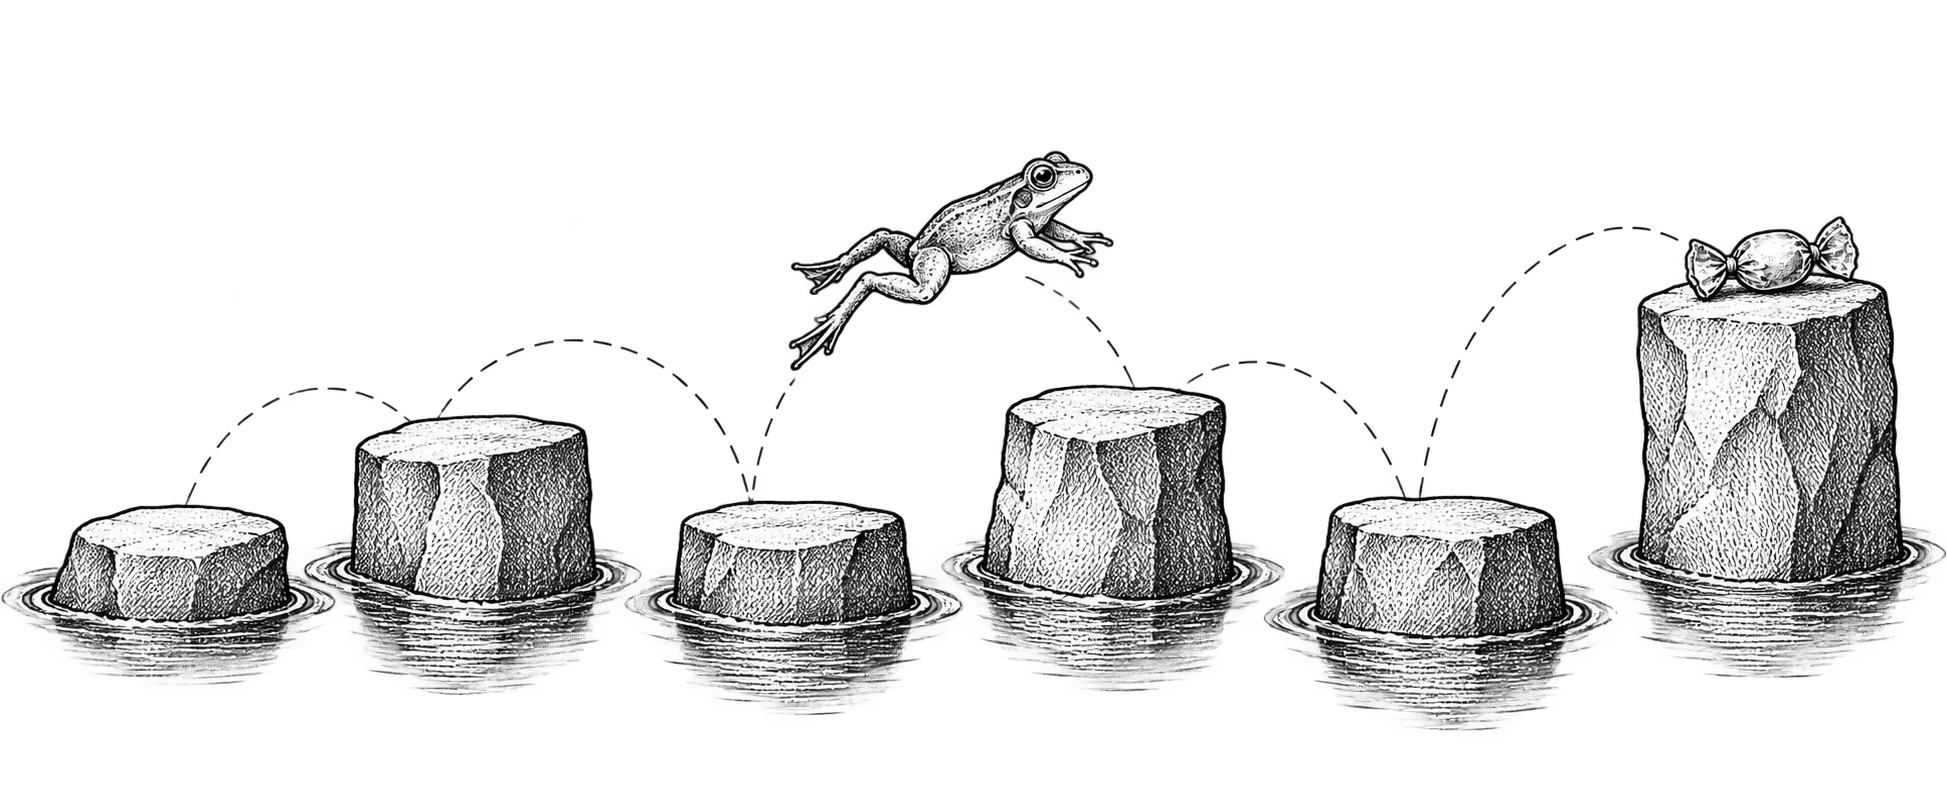
\includegraphics[width=174mm,height=94mm,keepaspectratio]{assets/cover.png}};
\node[anchor=north west,inner sep=0,text width=174mm] at ([xshift=18mm,yshift=-224mm]current page.north west)
{\fontsize{12}{16}\selectfont Understand what each step establishes\\and why it leads to the next.};
\node[anchor=west,inner sep=0] at ([xshift=18mm,yshift=-269mm]current page.north west)
{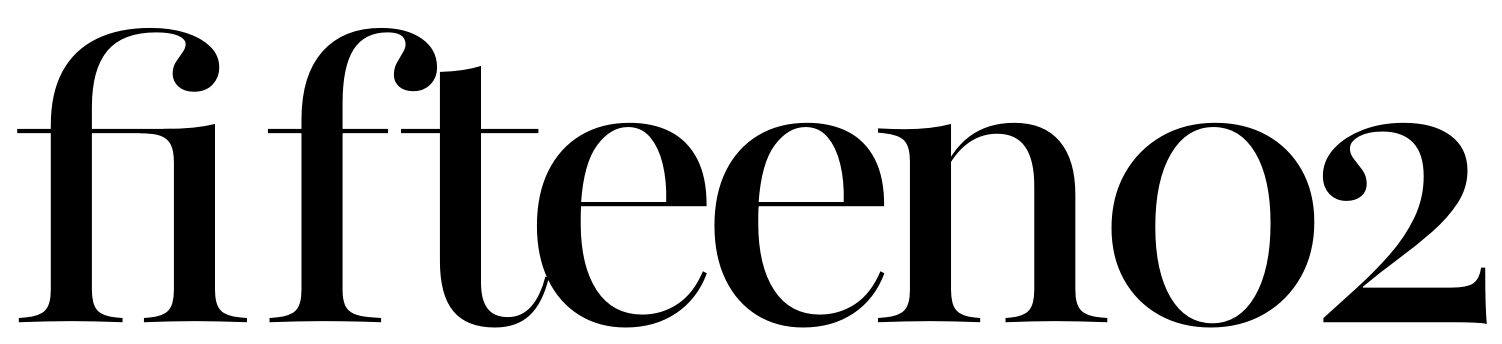
\includegraphics[width=43mm]{assets/logo.png}};
\node[anchor=east,inner sep=0] at ([xshift=192mm,yshift=-269mm]current page.north west)
{
\includegraphics[width=62mm]{assets/julians-pathfinder-monochrome.pdf}};
\node[anchor=north west,inner sep=0,text width=174mm] at ([xshift=18mm,yshift=-244mm]current page.north west) {\fontsize{11}{14}\selectfont \href{https://colab.research.google.com/github/fifteen02/julians-pathfinder/blob/main/Lesson\%201/lesson.ipynb}{\underline{Open this lesson in Google Colab}}};
\end{tikzpicture}\clearpage
\markboth{Questions}{}\raggedbottom\setlength{\parskip}{4pt}
{\heavy\fontsize{16}{20}\selectfont Lesson 1 / Staircase and Frog\par}\medskip
\par\noindent\begin{minipage}{\linewidth}
{\heavy\fontsize{12}{15}\selectfont Warm-up: functions that call themselves\par}\medskip
\textbf{L1-01 / A function that calls itself}\par\smallskip A function may call itself on a smaller input. countdown(n) below prints n and then calls countdown(n - 1); when n is 0 it prints Go! and makes no further call. In the table, write every call that countdown(3) makes, in order, what that call prints and which call it makes next.\par
\par\smallskip\noindent\colorbox{codepaper}{\parbox{\dimexpr\linewidth-2\fboxsep\relax}{\small\ttfamily\raggedright def countdown(n):\\\hspace*{2.4em}if n == 0:\\\hspace*{4.8em}print('Go!')\\\hspace*{4.8em}return\\\hspace*{2.4em}print(n)\\\hspace*{2.4em}countdown(n - 1)}}\par
\par\smallskip \begingroup\small\setlength{\tabcolsep}{4pt}\renewcommand{\arraystretch}{1.35}\begin{tabularx}{\linewidth}{>{\raggedright\arraybackslash}X>{\raggedright\arraybackslash}X>{\raggedright\arraybackslash}X}\toprule\textbf{Call} & \textbf{Prints} & \textbf{Calls next}\\\midrule
countdown(3) &  & \\
 &  & \\
 &  & \\
 &  & \\
\bottomrule\end{tabularx}\endgroup\par\smallskip 
\end{minipage}\par\vspace{2mm}
\par\noindent\begin{minipage}{\linewidth}
\textbf{L1-02 / Wait for the smaller answer}\par\smallskip sum\_squares(n) returns 0 when n is 0; otherwise it returns n * n + sum\_squares(n - 1). A call cannot finish until the call it waits for has returned. Fill the table for sum\_squares(4), starting from the bottom row and working up. Write the addition for each returned value.\par
\par\smallskip\noindent\colorbox{codepaper}{\parbox{\dimexpr\linewidth-2\fboxsep\relax}{\small\ttfamily\raggedright def sum\_squares(n):\\\hspace*{2.4em}if n == 0:\\\hspace*{4.8em}return 0\\\hspace*{2.4em}return n * n + sum\_squares(n - 1)}}\par
\par\smallskip \begingroup\small\setlength{\tabcolsep}{4pt}\renewcommand{\arraystretch}{1.35}\begin{tabularx}{\linewidth}{>{\raggedright\arraybackslash}X>{\raggedright\arraybackslash}X>{\raggedright\arraybackslash}X}\toprule\textbf{Call} & \textbf{Waits for} & \textbf{Returns}\\\midrule
sum\_squares(4) &  & \\
sum\_squares(3) &  & \\
sum\_squares(2) &  & \\
sum\_squares(1) &  & \\
sum\_squares(0) & nothing & 0\\
\bottomrule\end{tabularx}\endgroup\par\smallskip 
\end{minipage}\par\vspace{2mm}
\par\noindent\begin{minipage}{\linewidth}
\textbf{L1-03 / Find the missing base case}\par\smallskip power2(n) below should return 2 to the power n: 2 multiplied by itself n times, so power2(3) should be 8. What happens when you call power2(3)? Which value of n can you answer directly, without a smaller call? Add that base case and check that power2(3) now returns 8.\par
\par\smallskip\noindent\colorbox{codepaper}{\parbox{\dimexpr\linewidth-2\fboxsep\relax}{\small\ttfamily\raggedright def power2(n):\\\hspace*{2.4em}return 2 * power2(n - 1)}}\par
\par\smallskip{\small\textbf{Start with:}}\par\smallskip\noindent\colorbox{codepaper}{\parbox{\dimexpr\linewidth-2\fboxsep\relax}{\small\ttfamily\raggedright def power2(n):\\\hspace*{2.4em}return None  \# Replace with your answer.}}\par
{\small\textbf{What each function returns.}\par power2(n): the integer 2 raised to the power n.\par }
{\small\textbf{Hints.}}\begin{itemize}\item Trace the inputs until they pass 0. Where should the chain stop?\item Check your repaired function on the stopping input before trying 3.\end{itemize}
\end{minipage}\par\vspace{2mm}
\par\noindent\begin{minipage}{\linewidth}
\textbf{L1-04 / Write a recursive function}\par\smallskip factorial(n) is the product 1 × 2 × ... × n, and factorial(0) is 1. Write factorial(n) recursively: first the base case, then one smaller call. Predict factorial(4) before running it. The staircase that follows uses the same pattern, with two smaller calls instead of one.\par
\par\smallskip{\small\textbf{Start with:}}\par\smallskip\noindent\colorbox{codepaper}{\parbox{\dimexpr\linewidth-2\fboxsep\relax}{\small\ttfamily\raggedright def factorial(n):\\\hspace*{2.4em}return None  \# Replace with your answer.}}\par
{\small\textbf{What each function returns.}\par factorial(n): the product of integers 1 through n; for n = 0, return 1.\par }
{\small\textbf{Hints.}}\begin{itemize}\item What is the smallest n you can answer directly?\item If you already knew factorial(n - 1), what single step would give factorial(n)?\end{itemize}
\end{minipage}\par\vspace{2mm}
\par\noindent\begin{minipage}{\linewidth}
{\heavy\fontsize{12}{15}\selectfont Staircase: count, remember, then loop\par}\medskip
\textbf{L1-05 / Five steps, many routes}\par\smallskip Start on the ground, called step 0. Each move climbs exactly 1 or 2 steps. Count routes that land exactly on each target from step 1 to step 5. List the routes to step 5 as move lists, such as [1, 2, 2]. Does changing the order make a different route?\par
\par\smallskip \begingroup\small\setlength{\tabcolsep}{4pt}\renewcommand{\arraystretch}{1.35}\begin{tabularx}{\linewidth}{>{\raggedright\arraybackslash}X>{\raggedright\arraybackslash}X>{\raggedright\arraybackslash}X>{\raggedright\arraybackslash}X>{\raggedright\arraybackslash}X>{\raggedright\arraybackslash}X}\toprule\textbf{Step} & \textbf{1} & \textbf{2} & \textbf{3} & \textbf{4} & \textbf{5}\\\midrule
Routes &  &  &  &  & \\
\bottomrule\end{tabularx}\endgroup\par\smallskip 
\end{minipage}\par\vspace{2mm}
\par\noindent\begin{minipage}{\linewidth}
\textbf{L1-06 / The last move explains the sum}\par\smallskip The next move must land on step 5. Where can that move start? Use your L1-05 counts for step 4 and step 3. How can these two counts give the answer for step 5?\par
\end{minipage}\par\vspace{2mm}
\par\noindent\begin{minipage}{\linewidth}
\textbf{L1-07 / Where recursion stops}\par\smallskip Let ways(n) return the number of routes from the ground to target step n, using jumps of 1 or 2. What should ways(0) and ways(-1) return? Use these answers to work out ways(1).\par
\end{minipage}\par\vspace{2mm}
\par\noindent\begin{minipage}{\linewidth}
\textbf{L1-08 / The slow recursive program}\par\smallskip Write stairs\_slow(n), the number of staircase routes to step n with jumps of 1 or 2. Start with the stopping cases, then ask about the two possible starting steps of the final jump. Draw every call made for stairs\_slow(3) and write the returned count beside it.\par
\par\smallskip{\small\textbf{Start with:}}\par\smallskip\noindent\colorbox{codepaper}{\parbox{\dimexpr\linewidth-2\fboxsep\relax}{\small\ttfamily\raggedright def stairs\_slow(n):\\\hspace*{2.4em}return None  \# Replace with your answer.}}\par
{\small\textbf{What each function returns.}\par stairs\_slow(n): the number of ordered routes to step n using jumps of 1 or 2.\par }
{\small\textbf{Hints.}}\begin{itemize}\item Which targets can you answer without a smaller call? Think about 0 and about negative targets.\item The last move is 1 or 2 steps. Which smaller targets do those leave?\end{itemize}
\end{minipage}\par\vspace{2mm}
\par\noindent\begin{minipage}{\linewidth}
\textbf{L1-09 / Repeated questions in the call tree}\par\smallskip The diagram shows the first three levels of calls made while counting routes to step 5. Circle calls with the same input. What work does the second call to ways(3) repeat?\par
\begin{center}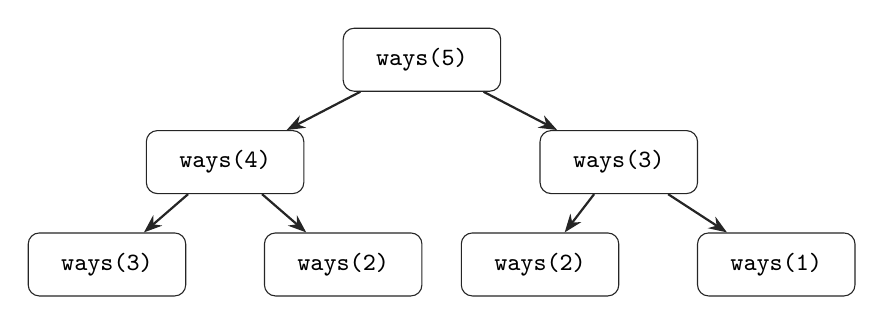
\begin{tikzpicture}[>=Stealth,every node/.style={font=\small},box/.style={draw=teal,rounded corners,minimum width=20mm,minimum height=8mm,fill=paper},arr/.style={->,thick,teal}]\node[box,fill=paper] (a) at (5,0) {\texttt{ways(5)}};\node[box,fill=paper] (b) at (2.5,-1.3) {\texttt{ways(4)}};\node[box,fill=paper] (c) at (7.5,-1.3) {\texttt{ways(3)}};\node[box,fill=paper] (d) at (1,-2.6) {\texttt{ways(3)}};\node[box,fill=paper] (e) at (4,-2.6) {\texttt{ways(2)}};\node[box,fill=paper] (f) at (6.5,-2.6) {\texttt{ways(2)}};\node[box,fill=paper] (g) at (9.5,-2.6) {\texttt{ways(1)}};\draw[arr] (a)--(b);\draw[arr] (a)--(c);\draw[arr] (b)--(d);\draw[arr] (b)--(e);\draw[arr] (c)--(f);\draw[arr] (c)--(g);\end{tikzpicture}\end{center}
\end{minipage}\par\vspace{2mm}
\par\noindent\begin{minipage}{\linewidth}
\textbf{L1-10 / A cache keeps an answer}\par\smallskip A cache is a dictionary that saves an answer under the input that produced it. We have found 5 routes to step 4. Complete cache[?] = ?. What should a later call to ways(4) return, and which work can it skip?\par
\end{minipage}\par\vspace{2mm}
\par\noindent\begin{minipage}{\linewidth}
\textbf{L1-11 / Fast work can still mean deep recursion}\par\smallskip Caching removes repeated work. Why can a large staircase input still cause RecursionError in Python? What does iteration change?\par
\end{minipage}\par\vspace{2mm}
\par\noindent\begin{minipage}{\linewidth}
\textbf{L1-12 / Build the table in order}\par\smallskip Write stairs\_table(n) using a loop. First fill ways[step], the route count, for steps 0 through 5. Which earlier count is available at step 1? Which two are needed from step 2 onwards? Use that order in your code.\par
\par\smallskip{\small\textbf{Start with:}}\par\smallskip\noindent\colorbox{codepaper}{\parbox{\dimexpr\linewidth-2\fboxsep\relax}{\small\ttfamily\raggedright def stairs\_table(n):\\\hspace*{2.4em}return None  \# Replace with your answer.}}\par
{\small\textbf{What each function returns.}\par stairs\_table(n): the number of ordered routes to step n using jumps of 1 or 2.\par }
{\small\textbf{Hints.}}\begin{itemize}\item How long must the list be so that ways[n] exists?\item Which entry do you know before the loop starts?\item When you fill ways[step], which entries must already be filled?\end{itemize}
\par\smallskip \begingroup\small\setlength{\tabcolsep}{4pt}\renewcommand{\arraystretch}{1.35}\begin{tabularx}{\linewidth}{>{\raggedright\arraybackslash}l>{\raggedright\arraybackslash}X>{\raggedright\arraybackslash}X>{\raggedright\arraybackslash}X>{\raggedright\arraybackslash}X>{\raggedright\arraybackslash}X>{\raggedright\arraybackslash}X}\toprule\textbf{Step} & \textbf{0} & \textbf{1} & \textbf{2} & \textbf{3} & \textbf{4} & \textbf{5}\\\midrule
ways[step] & 1 & ? & ? & ? & ? & ?\\
\bottomrule\end{tabularx}\endgroup\par\smallskip 
\end{minipage}\par\vspace{2mm}
\par\noindent\begin{minipage}{\linewidth}
\textbf{L1-13 / Your turn: jumps of 1 or 3}\par\smallskip Write stairs\_13(n) by adapting stairs\_table from L1-12. Allow only jumps of 1 or 3, never 2. First fill the counts for steps 0 through 7, then write and test your code.\par
\par\smallskip{\small\textbf{Start with:}}\par\smallskip\noindent\colorbox{codepaper}{\parbox{\dimexpr\linewidth-2\fboxsep\relax}{\small\ttfamily\raggedright def stairs\_13(n):\\\hspace*{2.4em}return None  \# Replace with your answer.}}\par
{\small\textbf{What each function returns.}\par stairs\_13(n): the number of ordered routes to step n using jumps of 1 or 3.\par }
{\small\textbf{Hints.}}\begin{itemize}\item Which line of stairs\_table depends on the allowed jumps?\item A jump can only start from a step that exists. What must be true before you read an earlier entry?\end{itemize}
\par\smallskip \begingroup\small\setlength{\tabcolsep}{4pt}\renewcommand{\arraystretch}{1.35}\begin{tabularx}{\linewidth}{>{\raggedright\arraybackslash}l>{\raggedright\arraybackslash}X>{\raggedright\arraybackslash}X>{\raggedright\arraybackslash}X>{\raggedright\arraybackslash}X>{\raggedright\arraybackslash}X>{\raggedright\arraybackslash}X>{\raggedright\arraybackslash}X>{\raggedright\arraybackslash}X}\toprule\textbf{Step} & \textbf{0} & \textbf{1} & \textbf{2} & \textbf{3} & \textbf{4} & \textbf{5} & \textbf{6} & \textbf{7}\\\midrule
ways[step] & 1 &  &  &  &  &  &  & \\
\bottomrule\end{tabularx}\endgroup\par\smallskip 
\end{minipage}\par\vspace{2mm}
\par\noindent\begin{minipage}{\linewidth}
{\heavy\fontsize{12}{15}\selectfont Frog: compare complete route costs\par}\medskip
\textbf{L1-14 / Frog: cost belongs to a whole route}\par\smallskip Number the stones 0, 1 and 2; their heights are [10, 20, 30]. A frog starts at stone 0 and may jump forward one or two positions. A jump costs the absolute height difference, so a drop of 10 also costs 10. List all routes to stone 2 and add the jump costs for each.\par
\end{minipage}\par\vspace{2mm}
\par\noindent\begin{minipage}{\linewidth}
\textbf{L1-15 / A greedy choice can fail}\par\smallskip Use heights [20, 50, 30, 40, 10, 10], at stones 0 through 5. At each stone, choose the cheaper of the next two legal jumps; if costs tie, choose the farther stone. Trace this greedy route and its total cost. Can another complete route cost less?\par
\par\smallskip \begingroup\small\setlength{\tabcolsep}{4pt}\renewcommand{\arraystretch}{1.35}\begin{tabularx}{\linewidth}{>{\raggedright\arraybackslash}l>{\raggedright\arraybackslash}X>{\raggedright\arraybackslash}X>{\raggedright\arraybackslash}X>{\raggedright\arraybackslash}X>{\raggedright\arraybackslash}X>{\raggedright\arraybackslash}X}\toprule\textbf{Stone i} & \textbf{0} & \textbf{1} & \textbf{2} & \textbf{3} & \textbf{4} & \textbf{5}\\\midrule
heights[i] & 20 & 50 & 30 & 40 & 10 & 10\\
\bottomrule\end{tabularx}\endgroup\par\smallskip 
\end{minipage}\par\vspace{2mm}
\par\noindent\begin{minipage}{\linewidth}
\textbf{L1-16 / Frog: ask about the last jump}\par\smallskip Write frog\_slow(heights) with recursive helper cost(i): the cheapest total cost from stone 0 to stone i. Which earlier stones can supply the last jump? Explore both possibilities.\par
\par\smallskip{\small\textbf{Start with:}}\par\smallskip\noindent\colorbox{codepaper}{\parbox{\dimexpr\linewidth-2\fboxsep\relax}{\small\ttfamily\raggedright def frog\_slow(heights):\\\hspace*{2.4em}def cost(i):\\\hspace*{4.8em}return None  \# Your helper goes here.\\\hspace*{2.4em}return cost(len(heights) - 1)}}\par
{\small\textbf{What each function returns.}\par frog\_slow(heights): the cheapest total cost from stone 0 to the last stone.\par cost(i): the cheapest total cost from stone 0 to stone i, including all jumps along the route.\par }
{\small\textbf{Hints.}}\begin{itemize}\item What is the smallest i you can answer directly?\item Which earlier stones can the last jump into stone i start from?\item What does cost(i) need to know about each of those stones?\end{itemize}
\end{minipage}\par\vspace{2mm}
\par\noindent\begin{minipage}{\linewidth}
\textbf{L1-17 / Frog: cache the stone number}\par\smallskip In the recursive Frog solution, what is the cache key? Why can different routes that reach the same stone share an answer?\par
\end{minipage}\par\vspace{2mm}
\par\noindent\begin{minipage}{\linewidth}
\textbf{L1-18 / Frog: write the iterative solution}\par\smallskip Write frog\_table(heights) using a loop. Return the cheapest total cost from stone 0 to the last stone. First fill best[i] for heights [20, 50, 30, 40, 10, 10], then turn those steps into Python code. Explain why the loop runs from left to right. Test your function on these heights.\par
\par\smallskip{\small\textbf{Start with:}}\par\smallskip\noindent\colorbox{codepaper}{\parbox{\dimexpr\linewidth-2\fboxsep\relax}{\small\ttfamily\raggedright def frog\_table(heights):\\\hspace*{2.4em}return None  \# Replace with your answer.}}\par
{\small\textbf{What each function returns.}\par frog\_table(heights): the cheapest total cost from stone 0 to the last stone.\par }
{\small\textbf{Hints.}}\begin{itemize}\item What is best[0], before any jump?\item Which earlier entries does best[i] need, and are they filled when the loop reaches i?\end{itemize}
\par\smallskip \begingroup\small\setlength{\tabcolsep}{4pt}\renewcommand{\arraystretch}{1.35}\begin{tabularx}{\linewidth}{>{\raggedright\arraybackslash}l>{\raggedright\arraybackslash}X>{\raggedright\arraybackslash}X>{\raggedright\arraybackslash}X>{\raggedright\arraybackslash}X>{\raggedright\arraybackslash}X>{\raggedright\arraybackslash}X}\toprule\textbf{Stone i} & \textbf{0} & \textbf{1} & \textbf{2} & \textbf{3} & \textbf{4} & \textbf{5}\\\midrule
heights[i] & 20 & 50 & 30 & 40 & 10 & 10\\
best[i] & 0 & ? & ? & ? & ? & ?\\
\bottomrule\end{tabularx}\endgroup\par\smallskip 
\end{minipage}\par\vspace{2mm}
\par\noindent\begin{minipage}{\linewidth}
\textbf{L1-19 / Your turn: a new Frog instance}\par\smallskip Test your frog\_table(heights) from L1-18. For heights [10, 30, 20, 40], first predict best[i] and give one cheapest route, then run your function. Next predict and test the answer for 100,000 equal-height stones. Explain why uncached recursion is unsuitable for that large test.\par
\par\smallskip \begingroup\small\setlength{\tabcolsep}{4pt}\renewcommand{\arraystretch}{1.35}\begin{tabularx}{\linewidth}{>{\raggedright\arraybackslash}X>{\raggedright\arraybackslash}X>{\raggedright\arraybackslash}X>{\raggedright\arraybackslash}X>{\raggedright\arraybackslash}X}\toprule\textbf{Stone i} & \textbf{0} & \textbf{1} & \textbf{2} & \textbf{3}\\\midrule
heights[i] & 10 & 30 & 20 & 40\\
best[i] & 0 &  &  & \\
\bottomrule\end{tabularx}\endgroup\par\smallskip 
\end{minipage}\par\vspace{2mm}
\par\noindent\begin{minipage}{\linewidth}
\textbf{L1-20 / Counting and minimising}\par\smallskip Both staircase and Frog inspect earlier states. Why does staircase add their answers, while Frog takes a minimum? What does each table entry mean?\par
\end{minipage}\par\vspace{2mm}
\par\noindent\begin{minipage}{\linewidth}
{\heavy\fontsize{12}{15}\selectfont Extension: recover a cheapest Frog route\par}\medskip
\textbf{L1-21 / OPTIONAL EXTENSION / Frog: recover a cheapest path}\par\smallskip Extend your cost solution: write frog\_path(heights), returning (cost, path), where path lists stone indices from start to finish. For heights [20, 50, 30, 40, 10, 10], record in previous[i] which earlier stone gives best[i]. Use -1 for the start. On equal costs keep i - 1. Trace backwards from the last stone, then return the path in forward order.\par
\par\smallskip{\small\textbf{Start with:}}\par\smallskip\noindent\colorbox{codepaper}{\parbox{\dimexpr\linewidth-2\fboxsep\relax}{\small\ttfamily\raggedright def frog\_path(heights):\\\hspace*{2.4em}return None  \# Replace with your answer.}}\par
{\small\textbf{What each function returns.}\par frog\_path(heights): a pair (cost, path): the minimum total cost and a list of stone indices from 0 to the last stone. On equal candidate costs, keep the predecessor i - 1.\par }
{\small\textbf{Hints.}}\begin{itemize}\item When a candidate becomes the cheapest, what earlier stone should you remember?\item Start at the last stone and follow the saved indices. How will you recognise the start?\item In which order did you collect the stones, and which order should you return?\end{itemize}
\par\smallskip\resizebox{\linewidth}{!}{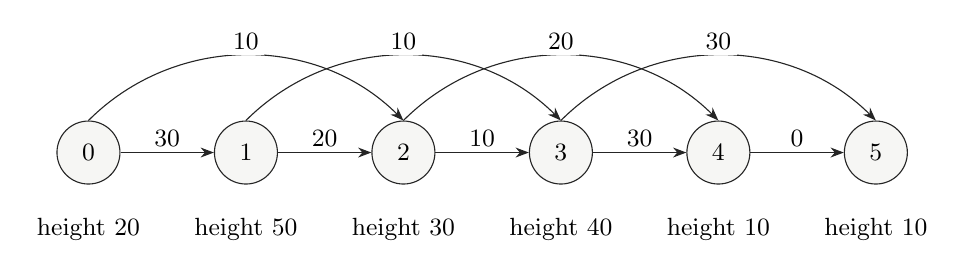
\begin{tikzpicture}[x=1cm,y=1cm,>=Stealth,every node/.style={font=\small}]
\node[draw=ink,circle,minimum size=8mm,fill=codepaper] (g0) at (0,0) {0};
\node[below=3mm] at (g0.south) {height 20};
\node[draw=ink,circle,minimum size=8mm,fill=codepaper] (g1) at (2,0) {1};
\node[below=3mm] at (g1.south) {height 50};
\node[draw=ink,circle,minimum size=8mm,fill=codepaper] (g2) at (4,0) {2};
\node[below=3mm] at (g2.south) {height 30};
\node[draw=ink,circle,minimum size=8mm,fill=codepaper] (g3) at (6,0) {3};
\node[below=3mm] at (g3.south) {height 40};
\node[draw=ink,circle,minimum size=8mm,fill=codepaper] (g4) at (8,0) {4};
\node[below=3mm] at (g4.south) {height 10};
\node[draw=ink,circle,minimum size=8mm,fill=codepaper] (g5) at (10,0) {5};
\node[below=3mm] at (g5.south) {height 10};
\draw[->,draw=ink] (g0.east) -- node[above,fill=white,inner sep=2pt] {30} (g1.west);
\draw[->,draw=ink] (g0.north) to[bend left=45] node[above,fill=white,inner sep=2pt] {10} (g2.north);
\draw[->,draw=ink] (g1.east) -- node[above,fill=white,inner sep=2pt] {20} (g2.west);
\draw[->,draw=ink] (g1.north) to[bend left=45] node[above,fill=white,inner sep=2pt] {10} (g3.north);
\draw[->,draw=ink] (g2.east) -- node[above,fill=white,inner sep=2pt] {10} (g3.west);
\draw[->,draw=ink] (g2.north) to[bend left=45] node[above,fill=white,inner sep=2pt] {20} (g4.north);
\draw[->,draw=ink] (g3.east) -- node[above,fill=white,inner sep=2pt] {30} (g4.west);
\draw[->,draw=ink] (g3.north) to[bend left=45] node[above,fill=white,inner sep=2pt] {30} (g5.north);
\draw[->,draw=ink] (g4.east) -- node[above,fill=white,inner sep=2pt] {0} (g5.west);
\end{tikzpicture}}\par Circles show stone indices; the height is below each circle. Each arrow is a legal jump, labelled with its cost. Mark the route returned by your program.
\end{minipage}\par\vspace{2mm}
\end{document}